\documentclass{article}

\usepackage{amsmath}
\usepackage{fancyhdr}
\usepackage{graphicx}
\graphicspath{{}}
\usepackage{placeins}
\usepackage{hyperref}
\usepackage[utf8]{inputenc}
\usepackage[margin=1in]{geometry}
\usepackage{titling}
\usepackage{datenumber}

\usepackage{minted}

%% some colours
\usepackage{xcolor}
\definecolor{deepblue}{rgb}{0,0,0.5}
\definecolor{deepred}{rgb}{0.6,0,0}
\definecolor{deepgreen}{rgb}{0,0.5,0}
\definecolor{backcolour}{rgb}{0.95,0.96,0.93}

%%%%%%%%%%%%%% CODE STUFF %%%%%%%%%%%%%%
%%%%%%%%%%%%%%%%%%%%%%%%%%%%%%%%%%%%%%%%
\newminted{python}{frame=single, framesep=5pt, linenos=true}
\newminted[outputcode]{text}{frame=single, framesep=5pt}


%%%%%%%%%%%%%%%%%%%%%%%%%%%%%%%%%%%%%%%%
% setting the style for ex documents
\pagestyle{fancy}
\fancyhf{}
\fancyhead[L]{\thetitle}
\fancyhead[C]{}
\fancyhead[R]{\theauthor}
\renewcommand{\headrulewidth}{0.4pt} %obere Trennlinie
\fancyfoot[L]{Due: \thedate}
\fancyfoot[R]{\thepage} %Seitennummer
\renewcommand{\footrulewidth}{0.4pt}

% include solutions
\ifdef{\solutions}
    {\newenvironment{solution}{\noindent \textbf{Solution:}}{}}
    % adapted from https://tex.stackexchange.com/a/194146
    {\newenvironment{solution}{\setbox0=\vbox\bgroup}{\egroup\iffalse\box0\fi}}


% Python execution environment
\newenvironment{pyexec}[1]{\noindent \textbf{Output: }  #1}{}


\author{K.\ Groß \and M.\ Pömsl \and S.\ Selbach}

\AtBeginDocument{
    \date{\datedate}
    The deadline for this exercise sheet is \textbf{\datedayname, \thedate\ at 23:59 CEST.}
}


\title{BPP Exercise 8 -- Standard Library}
% {YYYY}{MM}{DD}
\setdate{2019}{06}{02}


\begin{document}

\section{Warm-Up (20 points)}

\noindent 1.1. Using \texttt{time}, print the number of seconds that have passed since January 1st 1970 00:00:00.

\vspace{1em}

\begin{solution}

\begin{pythoncode}

import time

print(time.time())

\end{pythoncode}

\end{solution}

\noindent 1.2. Using \texttt{os}, write a function \texttt{make\_absolute} that converts a relative path to an absolute one.

\vspace{1em}

\begin{solution}

\begin{pythoncode}

import os

def make_absolute(relative_path):
    """Makes a relative path absolute."""
    return os.getcwd() + "/" + relative_path

\end{pythoncode}

\end{solution}

\noindent 1.3. Using \texttt{math}, write two functions \texttt{calculate\_x} and \texttt{calculate\_y} that take an \texttt{int n} between 1 and 12 as an argument and return the respective value of the following formulas:

\vspace{1em}

\noindent $calculate\_x(n) = 3 * \sin{\frac{n * \pi}{6}}$

\vspace{1em}

\noindent $calculate\_y(n) = 3 * \cos{\frac{n * \pi}{6}}$

\vspace{1em}

\noindent \textbf{Background information (not relevant for the implementation):} 

\vspace{1em}

\noindent These functions calculate the x and y position of the label for hour \texttt{n} on a clock of radius 3. The x position of the hour 12 would e.g. be $3 * \sin{\frac{12 * \pi}{6}} = 3 * \sin{2 * \pi} = 0$ and the y position $3 * \cos{\frac{12 * \pi}{6}} = 3 * \cos{2 * \pi} = 3$.

\vspace{1em}

\begin{solution}

\begin{pythoncode}

from math import sin, cos, pi

def calculate_x(n):
    """Calculates the x position of hour n on the clock."""
    return 3 * sin((n * pi) / 6)

def calculate_y(n):
    """Calculates the y position of hour n on the clock."""
    return 3 * cos((n * pi) / 6)

\end{pythoncode}

\end{solution}

\section{os, sys (20 points)}

In the folder Homework Sheets/Resources on StudIP, you will find the file 08\_comp\_tree.zip. Download it and extract it. 

\vspace{1em}

\noindent 2.1. Familiarize yourself with the folder structure. Can you find the system behind the comparison tree? Briefly explain the rules in a file \texttt{comp\_tree\_explained.txt}.

\vspace{1em}

\begin{solution}

\noindent There are three layers of folders. The folders on the lowest layer are all named after numbers between 1 and 100, e.g. "26". The folders on the middle layer are either also named after numbers or after comparisons with one specific number, e.g. "larger\_than\_25". The folders on the top layer are all named after comparisons. There are three kinds of comparisons: "larger\_than", "smaller\_than" and "equals". \newline The numbers are sorted according to the comparisons, e.g. the folder "larger\_than\_50" contains only numbers that are larger than 50.

\end{solution}

\vspace{1em}

\noindent 2.2. Write a script \texttt{insert.py} that takes a number as a command-line argument and then creates a folder with this name in the correct position according to the existing folder structure. You should use \texttt{os.listdir()} and \texttt{os.mkdir()} for this, which both take a relative or absolute path as an argument.

\vspace{1em}

\noindent \textbf{Hint 1:} \texttt{sys.argv[0]} is the name of your own script, \texttt{sys.argv[1]} is the first command-line argument.

\noindent \textbf{Hint 2:} With the command \texttt{tree} in the terminal you can get an overview of the folder structure. A screenshot of this can also be found on StudIP in the folder Homework Sheets/Resources.

\vspace{1em}

\begin{solution}

\begin{pythoncode}

import sys
import os

def get_path(n):
    """Returns the path of n in a comp_tree structure."""

    rel_path = "comp_tree/"
        
    if n > 50:
        rel_path += "larger_than_50/"
        if n > 75:
            rel_path += "larger_than_75/"
        elif n < 75:
            rel_path += "smaller_than_75/"
        else:
            rel_path += "equals_75/"
    elif n < 50:
        rel_path += "smaller_than_50/"
        if n > 25:
            rel_path += "larger_than_25/"
        elif n < 25:
            rel_path += "smaller_than_25/"
        else:
            rel_path += "equals_25/"
    else:
        rel_path += "equals_50/"

    rel_path += str(n)

    return rel_path

    
n = int(sys.argv[1])
path = get_path(n)

os.mkdir(path)

\end{pythoncode}

\end{solution}

\section{copy, random, time (30 points)}

\noindent 3.1. Write a function \texttt{rand\_change} that takes a nested 3x3 2d list (meaning a list with three row lists in it which each have three elements in it) as an argument and returns a deep copy of it in which one randomly selected cell was assigned a random integer between 1 and 3. Cells are elements of row lists.

\vspace{1em}

\noindent \textbf{Example}:

\begin{pythoncode}

my_list = [[1, 1, 1], [1, 1, 1], [1, 1, 1]]

my_list = rand_change(my_list)

print(my_list)
# Output: [[1, 1, 1], [2, 1, 1], [1, 1, 1]]

\end{pythoncode}

\begin{solution}

\begin{pythoncode}

from copy import deepcopy
import random

def rand_change(array):
    """Returns a copy with one random cell changed."""
    array_copy = deepcopy(array)
    x = random.randint(0, 2)
    y = random.randint(0, 2)
    array_copy[x][y] = random.randint(1, 3)
    return array_copy

\end{pythoncode}

\end{solution}

\noindent 3.2. Write a function \texttt{get\_diff} that takes two nested 3x3 2d lists and returns the number of how many cells (in the same x, y position) have different values.

\vspace{1em}

\noindent \textbf{Example}:

\begin{pythoncode}

list_1 = [[1, 1, 1], [1, 1, 1], [2, 3, 1]]

list_2 = [[3, 3, 3], [3, 3, 3], [1, 2, 3]]

print(get_diff(list_1, list_2))
# Output: 3

\end{pythoncode}

\begin{solution}

\begin{pythoncode}

def get_diff(array_1, array_2):
    """Returns the number of cells that differ."""
    diff = 0
    for x in range(3):
        for y in range(3):
            if array_1[x][y] != array_2[x][y]:
                diff += 1
    return diff

\end{pythoncode}

\end{solution}

\noindent 3.3. Create two nested 3x3 2d lists \texttt{ones} and \texttt{threes}. \texttt{ones} should be filled with value 1, \texttt{threes} should be filled with the value 3. Change both 2d lists with \texttt{rand\_change} until \texttt{get\_diff(ones, threes)} returns 0. Measure the time this took in seconds and print it.

\vspace{1em}

\noindent \textbf{Hint 1:} In the beginning, \texttt{get\_diff(ones, threes)} should return 9.

\noindent \textbf{Hint 2:} This should take at most 10 seconds. If it takes longer, you made a mistake somewhere.

\vspace{1em}

\begin{solution}

\begin{pythoncode}

# record start time
start = time.time()

ones = []
threes = []

# fill ones and threes
for x in range(3):
    row_ones = []
    row_threes = []
    for y in range(3):
        row_ones.append(1)
        row_threes.append(3)
    ones.append(row_ones)
    threes.append(row_threes)

diff = 1

while diff > 0:
    diff = get_diff(ones, threes)
    ones = rand_change(ones)
    threes = rand_change(threes)

# print time difference in seconds
print("It took {:.4f} seconds".format(time.time() - start))

\end{pythoncode}

\end{solution}

\section{math, time (30 points)}

To test our skills, we will implement a simplified formula for the increase in global temperature levels due to the radiative forcing of CO2 level changes.

\vspace{1em}

\noindent \textbf{Keep in mind that the following is an extremely simplified model which may be outdated and might not represent the current scientific consensus.}

\vspace{1em}

\noindent \textbf{Radiative forcing due to change in CO2 level:}\qquad \qquad \qquad $\Delta F = \alpha * ln(\frac{c_1}{c_0})$

\vspace{1em}

\noindent \textbf{Relation between radiative forcing and temperature:} \qquad $\lambda = \frac{\Delta T}{\Delta F}$

\vspace{1em}

\noindent $\alpha$ is fixed at 5.35 while $\lambda$ differs from model to model - we will simply use 0.5.

\vspace{1em}

\noindent $c_1$ denotes the changed CO2 level, $c_0$ denotes the unchanged CO2 level.

\vspace{1em}

\noindent Let's take the CO2 level of January 1970 as the unchanged CO2 level, so $c_0 = 325.03$. 

\vspace{1em}

\noindent Current levels of CO2 were at $c_1 = 411.97$ as of March 2019. We will just assume that the CO2 level has not changed significantly since then for the purposes of our calculations.

\vspace{1em}

\noindent This would result in a 0.63 K increase in global temperature since 1970, which is consistent with the actual change in global temperature, especially considering that there are also other influences on the global climate such as other greenhouse gases.

\vspace{1em}

\noindent \textbf{Your task is to do the following:} 

    \begin{enumerate}

        \item Calculate how many hours have passed since January 1st 1970 00:00:00
        \item Use this time difference to calculate the average CO2 increase per hour since 1970
        \item Use this CO2 increase per hour to calculate a projection of what the CO2 level could be in 2100 (assuming that the CO2 increase per hour stays constant)
        \item Calculate the increase in temperature in from 1970 to 2100 (use your projected CO2 level as $c_1$ and the value from 1970 as $c_0$)
        \item Now generalize steps 3. and 4. by writing a function \texttt{predict\_increase} that takes an \texttt{int year} larger than 1970 as an input and returns the increase in temperature from 1970 to \texttt{year}

    \end{enumerate}

\vspace{1em}

\begin{solution}

\begin{pythoncode}

from math import log
import time

co2_1970 = 325.03
co2_now = 411.97

alph = 5.35
lamb = 0.5

# hours that have passed since 1970
hours_passed_now = time.time() / 3600

# co2 increase since 1970
co2_increase_now = co2_now - co2_1970

# average co2 increase per hour since 1970
avg_co2_increase = co2_increase_now / hours_passed_now

# hours that have passed between 1970 and 2100
hours_passed_2100 = (2100 - 1970) * 365.25 * 24

# co2 level projection for 2100
co2_2100 = co2_1970 + (hours_passed_2100 * avg_co2_increase)

print("Projected CO2 level in 2100: {:.4f}".format(co2_2100))

# calculate change in radiative forcing
delta_F_2100 = alph * log(co2_2100 / co2_1970)

# calculate change in temperature
delta_T_2100 = lamb * delta_F_2100

print("Projected temperature increase from 1970 to 2100: {:.4f}".format(delta_T_2100))

def predict_increase(year):
    """Predicts the increase in temperature between 1970 and a given year."""

    # calculate projected value of co2 in year
    hours_passed = (year - 1970) * 365.25 * 24
    co2 = co2_1970 + (hours_passed * avg_co2_increase)
    
    # calculate temperature increase from 1970 to year
    delta_F = alph * log(co2 / co2_1970)
    delta_T = lamb * delta_F

    print("Projected temperature increase from 1970 to {}: {:.4f}".format(year, delta_T))

    
\end{pythoncode}

\end{solution}

\section{Bonus Task: map, plot (1 bonus point)}

This task will give a short impression on functional programming in python. For this, have a look at the build in function \texttt{map} at \href{https://docs.python.org/3/library/functions.html}{https://docs.python.org/3/library/functions.html}

\vspace{1em}

\noindent \textbf{Your task is to do the following:} 

    \begin{enumerate}

        \item Write a function \texttt{temp\_increase} that takes a number of hours as input and returns the increase in CO2 from 1970 until the given amount of hours. Again, assume that the average increase in CO2 per hour, that you have calculated in \textbf{4.1}, stays constant.
        \item Write a function \texttt{plot\_increase} that takes a year as input and makes a lineplot. 
        \item On the x-axis there have to be the hours, starting from zero in 1970 and then going onward until the given year is reached.
        \item For calculating the y-values, you have to use \texttt{temp\_increase} and \texttt{map}.

    \end{enumerate}

\vspace{1em}

\noindent \textbf{Example}:

\begin{pythoncode}

#plot the CO2 increase for every hour until 2100
plot_increase(2100)

\end{pythoncode}

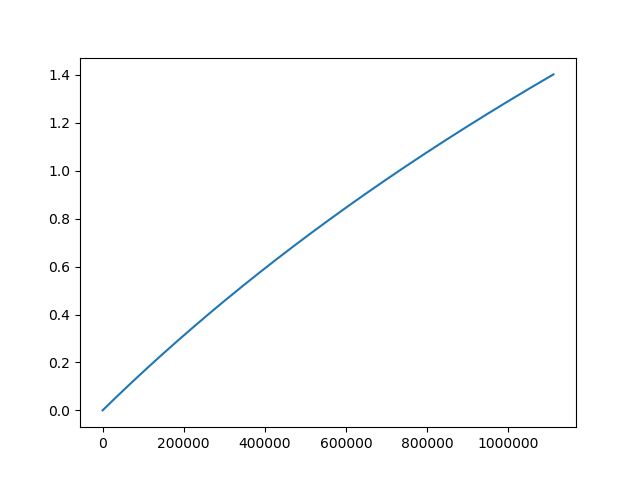
\includegraphics[width=10cm]{08_Standard_Library/temperature_2100.png}

\vspace{1em}

\noindent \textit{Formulas taken from: } IPCC (2001) Radiative Forcing of Climate Change, in Climate Change 2001: The Scientific Basis. Contribution of Working Group 1 to the Third Assessment. Report of the Intergovernmental Panel on Climate Change, CUP, pp. 349-416

\vspace{1em}

\noindent \textit{CO2 values taken from: } Dr. Pieter Tans, NOAA/ESRL (www.esrl.noaa.gov/gmd/ccgg/trends/) and Dr. Ralph Keeling, Scripps Institution of Oceanography. \url{https://www.esrl.noaa.gov/gmd/ccgg/trends/data.html}

\vspace{1em}

\begin{solution}

\begin{pythoncode}

import matplotlib.pyplot as plt
from math import log
import time

#define our constants
ALPHA = 5.35
LAMBDA = 0.5

#Here a non-pythonic notation was choosen, in order to stick to formula
c_0 = 325.03
c_1 = 415.88

#The average increase in CO2 is assumed to be constant
AVERAGE_INCREASE = (c_1 - c_0)/(time.time()/60/60)

def temp_increase(hours):
    """Calculates the increase in global temperature after a given
    amount of hours, based on the formula from the exercise sheet and
    under the assumption of a constant increase in CO2, given in
    ppm/hour
    """

    """It is ok to access constants from within functions. This should
    not be done with variables. Alternatively constants can be given as
    default values for arguments
    """
    co2_increase = hours*AVERAGE_INCREASE
    rad_forcing = ALPHA*log((c_0+co2_increase)/c_0)
    return rad_forcing*LAMBDA

def plot_increase(year):
    """Plots the increase in temperature against the hours, that have
    passed since 1/1/1970
    """

    #create x values: the hours that have passed
    x = range(int((year-1970)*356.25*24))

    #Use map in order to apply the function to every x value.
    y = list(map(temp_increase, x))

    #plot results
    plt.plot(x,y)
    plt.show()

#select some year
year = 2200

#call function
plot_increase(year)

"""The same thing as an awkwardly long oneliner, that combines all
functions in a so called lambda expression. Sticking to PEP makes
readability even worse in this case, so just never do stuff like 
this at home ;)
"""
plt.plot(range(int((year-1970)*356.25*24)), map(
    lambda x: LAMBDA*(ALPHA*log((c_0 + AVERAGE_INCREASE*x)/c_0)),
    range(int((year-1970)*356.25*24)))
                                               ))
plt.show()

\end{pythoncode}

\end{solution}

\end{document}
